\section{The \ruler~Benchmark}
\ruler~comprises tasks across four categories: \emph{retrieval}, \emph{multi-hop tracing}, \emph{aggregation}, and \emph{question answering}. Evaluation examples in \ruler~are automatically generated based on input configurations (see Table~\ref{tab:example-task}) that define the length and complexity of each input. Within a constrained domain as in RULER, the task complexity can be thought of as a function of the number of target output tokens and the signal-to-noise ratio in the context. We point readers to ~\citep{goldman2024really} for more comprehensive discussion on evaluation task design for long-context language models.

\begin{table}[t]
\centering
% \small
% \scalebox{0.99}{
\resizebox{0.99\linewidth}{!}{
\begin{tabular}[t]{@{}llp{0.8\linewidth}@{}}
\toprule
\textbf{Task} & \textbf{Configuration} & \textbf{Example} \\
\midrule
\begin{tabular}[t]{@{}l@{}}Single\\NIAH\\(S-NIAH)\end{tabular} & 
\begin{tabular}[t]{@{}l@{}}type\_key = word\\type\_value = number\\type\_haystack = essay\\size\_haystack $\propto$ context length\end{tabular} & 
\begin{tabular}[t]{@{}p{\linewidth}@{}}
\textcolor{lightgray}{(essays) ......} \\
One of the special magic numbers for \textcolor{violet}{long-context} is: \textcolor{orange}{12345}. \textcolor{lightgray}{......}  \\
What is the special magic number for \textcolor{violet}{long-context} mentioned in the provided text?\\
Answer: \textcolor{orange}{12345}
\end{tabular}
\\
\midrule
\begin{tabular}[t]{@{}l@{}}Multi-keys\\NIAH\\(MK-NIAH)\end{tabular}  &
\begin{tabular}[t]{@{}l@{}}num\_keys = 2\\type\_key = word\\type\_value = number\\type\_haystack = essay\\size\_haystack $\propto$ context length\end{tabular} & 
\begin{tabular}[t]{@{}p{\linewidth}@{}}
\textcolor{lightgray}{(essays) ......} \\ 
One of the special magic numbers for \textcolor{violet}{long-context} is: \textcolor{orange}{12345}. \\  
\textcolor{lightgray}{One of the special magic numbers for large-model is: 54321}. \\ 
\textcolor{lightgray}{......}  \\
What is the special magic number for \textcolor{violet}{long-context} mentioned in the provided text?\\
Answer: \textcolor{orange}{12345}
\end{tabular}
\\
\midrule
\begin{tabular}[t]{@{}l@{}}Multi-values\\NIAH\\(MV-NIAH)\end{tabular} &
\begin{tabular}[t]{@{}l@{}}num\_values = 2\\type\_key = word\\type\_value = number\\type\_haystack = essay\\size\_haystack $\propto$ context length\end{tabular} & 
\begin{tabular}[t]{@{}p{\linewidth}@{}}
\textcolor{lightgray}{(essays) ......} \\ 
One of the special magic numbers for \textcolor{violet}{long-context} is: \textcolor{orange}{12345}. \\  
One of the special magic numbers for \textcolor{violet}{long-context} is: \textcolor{orange}{54321}. \\  
\textcolor{lightgray}{......}  \\
What are all the special magic numbers for \textcolor{violet}{long-context} mentioned in the provided text?\\
Answer: \textcolor{orange}{12345}  \textcolor{orange}{54321}
\end{tabular}
\\
\midrule
\begin{tabular}[t]{@{}l@{}}Multi-queries\\NIAH\\(MQ-NIAH)\end{tabular} &
\begin{tabular}[t]{@{}l@{}}num\_queries = 2\\type\_key = word\\type\_value = number\\type\_haystack = essay\\size\_haystack $\propto$ context length\end{tabular} &  
\begin{tabular}[t]{@{}p{\linewidth}@{}}
\textcolor{lightgray}{(essays) ......} \\ 
One of the special magic numbers for \textcolor{violet}{long-context} is: \textcolor{orange}{12345}. \\  
One of the special magic numbers for \textcolor{violet}{large-model} is: \textcolor{orange}{54321}. \\  
\textcolor{lightgray}{......}  \\
What are all the special magic numbers for \textcolor{violet}{long-context} and \textcolor{violet}{large-model} mentioned in the provided text?\\
Answer: \textcolor{orange}{12345}  \textcolor{orange}{54321}
\end{tabular}
\\
\midrule
\begin{tabular}[t]{@{}l@{}}Variable\\Tracking\\(VT)\end{tabular} &
\begin{tabular}[t]{@{}l@{}}num\_chains = 2\\num\_hops = 2\\size\_noises $\propto$ context length\end{tabular} &
\begin{tabular}[t]{@{}p{\linewidth}@{}}
\textcolor{lightgray}{(noises) ......} \\
VAR \textcolor{orange}{X1} = \textcolor{violet}{12345} \textcolor{lightgray}{...... VAR Y1 = 54321 ......}  \\
VAR \textcolor{orange}{X2} = \textcolor{orange}{X1} \textcolor{lightgray}{...... VAR Y2 = Y1 ......} \\
VAR \textcolor{orange}{X3} = \textcolor{orange}{X2} \textcolor{lightgray}{...... VAR Y3 = Y2 ......} \\
Find all variables that are assigned the value \textcolor{violet}{12345}. \\
Answer: \textcolor{orange}{X1 X2 X3}
\end{tabular}
\\
\midrule
\begin{tabular}[t]{@{}l@{}}Common Words\\Extraction\\(CWE)\end{tabular} &
\begin{tabular}[t]{@{}l@{}}freq\_cw = 2, freq\_ucw = 1\\num\_cw = 10\\num\_ucw $\propto$ context length\end{tabular} & 
\begin{tabular}[t]{@{}p{\linewidth}@{}}
\textcolor{orange}{aaa} \textcolor{lightgray}{bbb} \textcolor{orange}{ccc} \textcolor{orange}{aaa} \textcolor{lightgray}{ddd} \textcolor{lightgray}{eee} \textcolor{orange}{ccc} \textcolor{lightgray}{fff} \textcolor{lightgray}{ggg} 
\textcolor{lightgray}{hhh} \textcolor{orange}{iii} \textcolor{orange}{iii} \textcolor{lightgray}{......}\\
What are the 10 most common words in the above list? \\
Answer: \textcolor{orange}{aaa ccc iii ......}
\end{tabular}
\\
\midrule
\begin{tabular}[t]{@{}l@{}}Frequent Words\\Extraction\\(FWE)\end{tabular} &
\begin{tabular}[t]{@{}l@{}}$\alpha$ = 2\\num\_word $\propto$ context length\end{tabular} & 
\begin{tabular}[t]{@{}p{\linewidth}@{}}
\textcolor{orange}{aaa} \textcolor{lightgray}{bbb} \textcolor{orange}{ccc} \textcolor{orange}{aaa} \textcolor{lightgray}{ddd} \textcolor{lightgray}{eee} \textcolor{orange}{ccc} \textcolor{lightgray}{fff} \textcolor{lightgray}{ggg} \textcolor{orange}{aaa} \textcolor{lightgray}{hhh} \textcolor{orange}{aaa} \textcolor{orange}{ccc} \textcolor{orange}{iii} \textcolor{orange}{iii}  \textcolor{lightgray}{......}\\
What are the 3 most frequently appeared words in the above coded text? \\
Answer: \textcolor{orange}{aaa ccc iii}
\end{tabular}
\\
\midrule
\begin{tabular}[t]{@{}l@{}}Question\\Answering\\(QA)\end{tabular} &
\begin{tabular}[t]{@{}l@{}}dataset = SQuAD\\num\_document $\propto$ context length\end{tabular} & 
\begin{tabular}[t]{@{}p{\linewidth}@{}}
\textcolor{lightgray}{Document 1: ...... aaa ......} \\
\textcolor{violet}{Document 2:} \textcolor{lightgray}{......} \textcolor{orange}{bbb} \textcolor{lightgray}{......} \\
\textcolor{lightgray}{Document 3: ...... ccc ......} \\
Question: \textcolor{violet}{question} \\
Answer: \textcolor{orange}{bbb}
\end{tabular}
\\
\bottomrule
\end{tabular}}
\caption{Task examples with flexible configurations in~\ruler. 
We use different colors to highlight \textcolor{violet}{queries}, \textcolor{violet}{keys}, \textcolor{orange}{values}, and \textcolor{lightgray}{distractors} in our examples.}
\label{tab:example-task}
\end{table}
\subsection{Retrieval: Needle-in-a-haystack (NIAH)} 

Recent works~\citep{gemini,claude200kprompting} commonly employ the needle-in-a-haystack~\citep[][NIAH]{needle} test to evaluate long-context modeling capability. The NIAH test is reminiscent of the extensively studied~\citep{Hopfield1982NeuralNA,neuralturingmachine,inductionhead,mqar} \emph{associative recall} tasks, in which relevant information needs to be retrieved from context given a sufficient query. In \ruler, we include multiple retrieval-based tasks, extending the vanilla NIAH test to evaluate models based on three criteria. Concretely, the retrieval capability should be (1) agnostic to the type of the ``needle'' and the ``haystack'', (2) strong enough to disregard hard distractors, and (3) of high recall when multiple items need to be retrieved. Based on these criteria, we develop four NIAH tasks. The ``needle'' in each of these tasks is a \emph{key-value} pair inserted into the ``haystack'' (long distractor texts). The \emph{query} is located at the end of the sequence and serves as a cue for matching the \emph{keys} in the context and subsequently retrieving the associated \emph{values}. 
\begin{itemize}[leftmargin=0.8em]
\itemsep0em 
\item \textbf{Single NIAH (S-NIAH): } This is the vanilla NIAH test where a single ``needle''\footnote{Similar to~\citet{lwm}, we use ``\emph{the special magic number for XXX is: YYY}'' as the needle due to its extendability instead of the sentence about San Francisco proposed by~\citet{needle}.} needs to be retrieved from the ``haystack''.
The \emph{query}/\emph{key}/\emph{value} can take the form of words, numbers (7 digits), or UUIDs (32 digits). The ``haystack'' can be repeated noise sentences\footnote{ Following~\citet{landmark}, we use ``\emph{The grass is green. The sky is blue. The sun is yellow. Here we go. There and back again.}'' as noise sentences.} or Paul Graham essays~\citep{needle}.

\item \textbf{Multi-keys NIAH (MK-NIAH): } Multiple ``needles'' are inserted into the ``haystack'', and only one of them needs to be retrieved. The additional ``needles'' are hard distractors. The most challenging setting is a version where the ``haystack'' is filled with distractor needles.

\item \textbf{Multi-values NIAH (MV-NIAH): } Multiple ``needles'' sharing the same \emph{key} are inserted into the ``haystack''. All \emph{values} associated with the same \emph{key} need to be retrieved. 

\item \textbf{Multi-queries NIAH (MQ-NIAH): } Multiple ``needles'' are inserted into the ``haystack''. All ``needles'' with distinct keys need to be retrieved. This is the same \emph{multi-query associative recall} task setup used by~\citet{mqar}. Together with MV-NIAH, these two tasks evaluate the retrieval capability without missing any critical information.
\end{itemize}

\subsection{Multi-hop Tracing: Variable Tracking (VT)} 

Effective discourse comprehension~\citep{dijkdiscourse} is contingent upon successful recognition of newly mentioned entities and establishing the chain of references co-referring to the same entity~\citep{discourse-referents} throughout the long context. We develop a new task \emph{variable tracking} to emulate a minimal coreference chain resolution~\citep{ng-2010-supervised} task. This task checks the behavior of tracking relevant co-occurrence patterns and drawing skipped connections within long input. Specifically, a variable $X1$ is initialized with a value $V$, followed by a linear \emph{chain} of variable name binding statements (e.g., $X2 = X1, X3 = X2, ...$), which are inserted at various positions of the input. The objective is to return \emph{all} variable names pointing to the same value $V$. The task complexity can be increased by adding more hops (i.e., the times of name binding) or more chains, similar to adding hard distractors in MK-NIAH. 


\subsection{Aggregation: Common Words (CWE) and Frequent Words Extraction (FWE)}
% The critical information (e.g., queried key-value pairs) in the previous two categories consists primarily of short strings, while most of the context functions as background noise. 
% spans long range of context, constitutes greater portion of the context, proxy for summarization task 
In \ruler, we introduce a new category as a  proxy for summarization tasks where relevant information constitutes much larger portion of the context, and the target output depends on accurate aggregation of the relevant input.
% In \ruler, we introduce a new category where the target output requires aggregating relevant information that spans long ranges in the context, . 
Concretely, we construct an input sequence by sampling words from a pre-defined (synthetic) word list. In the common word extraction task (CWE), words are sampled from discrete uniform distributions, with the number of common words fixed while the number of uncommon words increases with the sequence length. In the frequent words extraction task (FWE), words are sampled from Zeta distribution.\footnote{We draw inspiration from Zipf's Law~\citep{zipfslaw}. Let $N$ be the total number of words, which is determined by the context size, the frequency of the $k$-th ranked word (the $k$-th most frequently appeared word) is $\frac{k^{-\alpha}N}{\zeta(\alpha)}$, where $\zeta(\alpha)$ is the Zeta function. We set the top-ranked word to noise.} Figure~\ref{fig:AG_distribution} shows an illustration of word frequency in the constructed input. A model needs to return the top-$K$ frequent words in the context. In CWE, $K$ equals to the number of common words. In FWE, we set $K$ to 3, as increasing $K$ leads to poor performance even at small context sizes for most models.  The task complexity can be adjusted by varying the number of common words or the parameter of Zeta distribution. 

\begin{figure*}
    \centering
    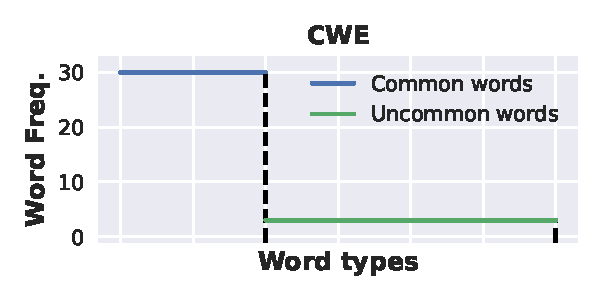
\includegraphics[width=0.4\linewidth]{Image/pdf/plot_uniform.pdf}
    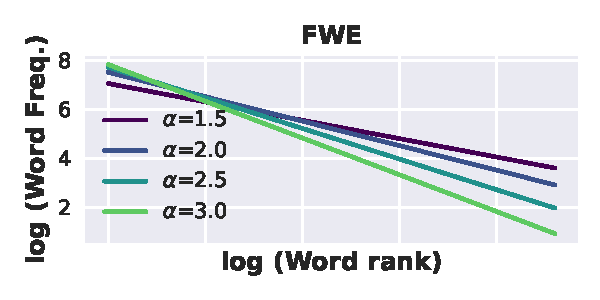
\includegraphics[width=0.4\linewidth]{Image/pdf/plot_zeta.pdf}
    \caption{In aggregation tasks, we sample words from a vocabulary following the two distributions above. The common words extraction (CWE) samples from uniform distributions. In the frequent words extraction (FWE), the frequency of each word is determined by its rank in the vocabulary and the parameter $\alpha$ of Zeta distribution.}
    \label{fig:AG_distribution}
\end{figure*}

\subsection{Question Answering (QA)}
The majority of existing QA datasets~\citep{squad, hotpotqa, musique} are designed to answer questions based on short passages. These datasets can be extended to simulate long-context input by adding distracting information. In this task category, we insert the golden paragraphs (i.e., the paragraphs that contain answers) into paragraphs randomly sampled from the same dataset. This category is a real-world adaptation~\citep{sled} of NIAH, where the question serves as the query, the golden paragraphs are the ``needles'', and the distracting paragraphs form the ``haystack''.
% These datasets can be easily extended to simulate long-context input by adding distracting information. 
% our approach involves constructing inputs through the concatenation of randomly sampled paragraphs with the original golden question-paragraphs pair. 
% The complexity of this task can be controlled by the selection of existing question answering datasets. 





% To be more specific, we can formulate this task as given a query, model should find the key matching the query and return the corresponding value in the gradually increased text distraction. With this definition, we have the flexibility to change the types and amounts of query, key, and value to formulate our proposed variants of NIAH, as listed in the following.

% \item \textbf{Multi-keys NIAH (MK-NIAH). } In single NIAH, we only have one needle in the haystack, so models can easily retrieve the needle based on the query. To make the test more complex, we introduce multi-keys NIAH by adding distracted needles in the haystack. The goal is to test whether model has the ability to locate a single key and ignore other similar needles. The configuration of this task is to increase the number of needle keys in the haystack. However, the most challenging setting is we fill the haystack with all distracted needles.

% \item \textbf{Multi-values NIAH (MV-NIAH). } Even if models can accurately ignore distracted needles and retrieve the correct single needle, our next goal is to test whether model has the ability to retrieve multiple values when there are multiple matched keys. This task can simulate the real-world use cases when users ask about a character information in a novel or a variable in a code base. The configuration of this task is to increase the number of needle values for each needle key.

% \item \textbf{Multi-queries NIAH (MQ-NIAH). } The next challenging task is when asking multiple queries in a single turn, models should locate all of the matched keys and retrieve the corresponding values. If we have the same keys for all needles, then this task can be viewed as multi-values NIAH. If we ask queries by one query in one turn, then this task can be adapted to multi-turn multi-keys NIAH. Although there are similarities, the goal is to test whether model has the ability to integrate multiple queries. The configuration of this task is to increase the number of needle queries in the question.

% To measure long context retrieval ability of a language model, people have evaluated on the needle-in-a-haystack task~\citep{lwm, gemini, yi} by retrieving a needle statement inserted in a random position of a sequence haystack~\citep{needle}. We can increase the size of haystack to measure whether model can have the same retrieval performance as length increases. 

% In this task, the goal is to test whether model has the ability to locate a single key and retrieve the corresponding value in a large distracted context. Since people~\citep{gemini} have found this task is too easy for existing models, we propose to change the types of needle and haystack to test model robustness of retrieval. For the needle, we can change the types of query-key and value to any text formats such as words (adjective-noun), numbers (7 digits), or UUIDs (32 digits). For the haystack, we can use repeated sentences \textit{The grass is green. The sky is blue. The sun is yellow. Here we go. There and back again.} following \citet{landmark} or concatenated essays written by Paul Graham following \citet{needle}.

% Our first task is the widely used passkey retrieval~\citep{landmark}, a variant of single NIAH with the word type key (adjective-noun) and number type value (7 digits) in the needle and repeated sentences ``The grass is green. The sky is blue. The sun is yellow. Here we go. There and back again.'' as the haystack. To make this task more difficult, we replace the repeated sentences with Paul Graham essays to mimic the haystack in real world format, referred to the well known vanilla single NIAH. Since people~\citep{gemini} have found these tasks are too easy for existing models, we propose to change the value type to test the model robustness of retrieving a UUID (32 digits) as a longer value sequence or a word as a more realistic value sequence. Total tasks for single NIAH are in the Appendix~\ref{appendix-s-niah}.

% We first add three extra needles into haystack as an initial test. Additionally, we introduce a harder task by filling the haystack with all distracted needles, similar to line retrieval~\citep{longchat}. To be more challenging,  we formulate each needle with key and value to be UUID type, similar to kv retrieval~\citep{lostmiddle}. These three tasks are in the Appendix~\ref{appendix-mk-niah}.

% Although we have the flexibility to increase task difficulties by increasing the amount of values, we only use two and four values for a needle key as two tasks respectively (see Appendix~\ref{appendix-mv-niah}). 

% Although we have the flexibility to increase task difficulties by increasing the amount of queries, we only use two and four queries in the question as two tasks respectively (see Appendix~\ref{appendix-mq-niah}).